
\documentclass[a4paper,UKenglish,cleveref, autoref, thm-restate]{lipics-v2021}
%This is a template for producing LIPIcs articles. 
%See lipics-v2021-authors-guidelines.pdf for further information.
%for A4 paper format use option "a4paper", for US-letter use option "letterpaper"
%for british hyphenation rules use option "UKenglish", for american hyphenation rules use option "USenglish"
%for section-numbered lemmas etc., use "numberwithinsect"
%for enabling cleveref support, use "cleveref"
%for enabling autoref support, use "autoref"
%for anonymousing the authors (e.g. for double-blind review), add "anonymous"
%for enabling thm-restate support, use "thm-restate"
%for enabling a two-column layout for the author/affilation part (only applicable for > 6 authors), use "authorcolumns"
%for producing a PDF according the PDF/A standard, add "pdfa"

% \usepackage{ltexpprt}
%\usepackage{footmisc}
\usepackage{hyperref}

% *** MATH PACKAGES ***
%
\usepackage{amsmath}
\usepackage{nicefrac}
\usepackage{array}
\usepackage{lmodern,amssymb}
\usepackage{float}
\usepackage{graphicx}
\usepackage{caption}
\usepackage{subcaption}
\usepackage{tikz}
\usetikzlibrary{positioning}
\usetikzlibrary{shapes.misc}
\usetikzlibrary{positioning, arrows.meta, shapes, fit, calc}

\usepackage[utf8]{inputenc}
\usepackage[T1]{fontenc}
% \usepackage[english]{babel}
\usepackage{pgfplots}
\usepackage{algorithm}
\usepackage{algpseudocode}
\usepackage{mathtools}
\usepackage{booktabs}

%\pdfoutput=1 %uncomment to ensure pdflatex processing (mandatatory e.g. to submit to arXiv)
%\hideLIPIcs  %uncomment to remove references to LIPIcs series (logo, DOI, ...), e.g. when preparing a pre-final version to be uploaded to arXiv or another public repository
\nolinenumbers

%\graphicspath{{./graphics/}}%helpful if your graphic files are in another directory

\bibliographystyle{plainurl}% the mandatory bibstyle

\title{Exact Lower Bounds for the Number of Comparisons in Selection}

%\titlerunning{Dummy short title} %TODO optional, please use if title is longer than one line

\author{Josua Dörrer}{University of Stuttgart, Germany}{}{}{}
\author{Konrad Gendle}{University of Stuttgart, Germany}{}{}{}
\author{Johanna Hofmann}{University of Stuttgart, Germany}{}{}{}
\author{Julius von Smercek}{University of Stuttgart, Germany}{}{}{}
\author{Andreas Steding}{University of Stuttgart, Germany}{}{}{}
\author{Florian Stober}{University of Stuttgart, Germany}{florian.stober@fmi.uni-stuttgart.de}{0000-0002-5516-6660}{}


\authorrunning{J.\ Dörrer, K.\ Gendle, J.\ Hofmann, J.\ von Smercek, A.\ Steding, F.\ Stober} 

\Copyright{Josua Dörrer, Konrad Gendle, Johanna Hofmann, Julius von Smercek, Andreas Steding, and Florian Stober} 

\ccsdesc[500]{Theory of computation~Sorting and searching}
\ccsdesc[300]{Mathematics of computing~Combinatorial algorithms}


\keywords{selection, lower bounds, exhaustive computer search}


\category{} %optional, e.g. invited paper

\relatedversion{} %optional, e.g. full version hosted on arXiv, HAL, or other respository/website
%\relatedversiondetails[linktext={opt. text shown instead of the URL}, cite=DBLP:books/mk/GrayR93]{Classification (e.g. Full Version, Extended Version, Previous Version}{URL to related version} %linktext and cite are optional

%\supplement{}%optional, e.g. related research data, source code, ... hosted on a repository like zenodo, figshare, GitHub, ...
%\supplementdetails[linktext={opt. text shown instead of the URL}, cite=DBLP:books/mk/GrayR93, subcategory={Description, Subcategory}, swhid={Software Heritage Identifier}]{General Classification (e.g. Software, Dataset, Model, ...)}{URL to related version} %linktext, cite, and subcategory are optional

%\funding{(Optional) general funding statement \dots}%optional, to capture a funding statement, which applies to all authors. Please enter author specific funding statements as fifth argument of the \author macro.

%\acknowledgements{I want to thank \dots}%optional

%\nolinenumbers %uncomment to disable line numbering



%Editor-only macros:: begin (do not touch as author)%%%%%%%%%%%%%%%%%%%%%%%%%%%%%%%%%%
\EventEditors{Petra Mutzel and Nicola Prezza}
\EventNoEds{2}
\EventLongTitle{23rd International Symposium on Experimental Algorithms (SEA 2025)}
\EventShortTitle{SEA 2025}
\EventAcronym{SEA}
\EventYear{2025}
\EventDate{July 22--24, 2025}
\EventLocation{Venice, Italy}
\EventLogo{}
\SeriesVolume{338}
\ArticleNo{3}
%%%%%%%%%%%%%%%%%%%%%%%%%%%%%%%%%%%%%%%%%%%%%%%%%%%%%%

% Commands
%! parser=off
\newcommand\smallO{
\mathchoice
{{\scriptstyle\mathcal{O}}}% \displaystyle
{{\scriptstyle\mathcal{O}}}% \textstyle
{{\scriptscriptstyle\mathcal{O}}}% \scriptstyle
{\scalebox{.50}{$\scriptscriptstyle\mathcal{O}$}}%\scriptscriptstyle
}
%! parser=on
\DeclareMathOperator{\N}{\mathbb{N}}
\newcommand{\set}[2]{\left\{\, \mathinner{#1}\vphantom{#2}\: \left|\: \vphantom{#1}\mathinner{#2} \right.\,\right\}}
\newcommand\ie{i.e\@., }
\newcommand{\sse}{\subseteq}
\newcommand{\pchild}[3]{{#1}\kern-1pt{+}{#2}{#3}}
\newcommand{\dual}[1]{{#1}^{\delta}}
\newcommand{\reduced}[1]{\operatorname{red}#1}
\newcommand{\less}[2]{D_{#1}(#2)}
\newcommand{\greater}[2]{U_{#1}(#2)}

\newcommand{\projectURL}[0]{https://github.com/JGDoerrer/selection_generator}
\newcommand{\projectServer}[0]{GitHub}

\supplement{}
\supplementdetails[subcategory={Source Code}, cite={}, swhid={}]{Software}{https://github.com/JGDoerrer/selection_generator}

\begin{document}

\maketitle
% // ===================================================

\begin{abstract} \small\baselineskip=9pt
  Selection is the problem of finding the $i$-th smallest element among $n$ elements.
  We apply computer search to find optimal algorithms for small instances of the selection problem.
  Using new algorithmic ideas, we establish tighter lower bounds for the number of comparisons required, denoted as $V_i(n)$.
  Our results include optimal algorithms for $n$ up to 15 and arbitrary $i$, and for $n=16$ when $i \leq 6$.
  We determine the precise values $V_7(14) = 25$, $V_6(15) = V_7(15) = 26$, and $V_8(15) = 27$, where previously, only a range was known.

\end{abstract} % newline above is important for formatting

\section{Motivation} \label{sec:motivation}

The problem of selecting the $i$-th smallest element in a list of $n$ elements is a well-known problem in computer science called \textit{selection}.
Explicitly, we concern ourselves with the optimal worst-case selection of a single element from a set of initially unordered unique elements, measuring the cost by the number of comparisons.
We denote this cost as $V_i(n)$.

For selecting the smallest element, optimal algorithms are known with $V_1(n) = n - 1$.
For the second smallest element, it is known that $V_2(n) = n - 2 + \lceil \log n\rceil$~\cite{Knuth1973} (all logarithms are to base $2$).
In general, the selection problem is solvable in linear time using the median of medians algorithm~\cite{Blum1972}.
Looking at the special case of selecting the median $i = \nicefrac{n}{2}$, the best-known algorithm requires $2.95n$ comparisons~\cite{dor1999selecting}.
For other values of $i$, the algorithm in~\cite{dor1999selecting} requires fewer comparisons, thus providing a general upper bound.
This presents a significant gap compared to the best-known lower bound, which is $\left (1 + H(\nicefrac{i}{n}) \right ) \cdot n + \Omega(\sqrt n)$, where $H(x) = x \cdot \log \frac{1}{x} + (1 - x) \log \frac{1}{1 - x}$~\cite{bent1985finding}.
For the median, this lower bound is $2 \cdot n - \smallO(n)$.
Paterson conjectured that the lower bound for selecting the median is $n \log_{4/3} 2 \approx 2.41n$~\cite{paterson1996progress}.
To improve these bounds toward tightness, it is essential to have known optimal reference points that general approaches can be compared against.

Gasarch, Kelly, and Pugh~\cite{Gasarch1996} were the first to use computer search to find optimal selection algorithms for fixed $n$ and $i$.
Oksanen continued this line of work, improving upon the previously known lower bounds~\cite{Oksanen2006}.
His results and the computer program he used to obtain them are available on his website~\cite{Oksanen}, but have not been published in a scientific journal.

We will also tackle the selection problem using computer search.
We reimplement the minimax algorithm used in~\cite{Gasarch1996,Oksanen,Oksanen2006} and improve upon it by introducing suitable heuristics.
Then we explore a different search strategy, the backward search, which is another significant improvement over the minimax algorithm.
A quote from Miguel de Cervantes from Don Quijote will hold true for this article: ``the journey is better than the inn''~\cite{cervantes_don_quijote}.
So buckle up.

\subsection{Contribution.}
In this work, we apply two different search algorithms to finding optimal algorithms for selection.
The first, which we will call forward search in the remainder of this article, is based on the minimax algorithm also used by Gasarch et.\ al\@.~\cite{Gasarch1996} and Oksanen~\cite{Oksanen,Oksanen2006}.
We introduce a novel pruning criterion based on the notion of compatible solutions, and demonstrate that this leads to a significant improvement compared to the benchmark implementation from~\cite{Oksanen}.

The second algorithm, the backward search, is based on an entirely different idea.
Here, the start and endpoint of the search switch places.
This type of search has not been applied to the selection problem before, and its efficient application poses several challenges, the solution of which is the main technical contribution of this work.

One such challenge is the use of reduced posets.
A poset is reduced by removing all elements that cannot be the $i$-th smallest.
In the forward search this is a straightforward optimization to reduce the search space.
To apply this optimization in the backward search, we show that reduced posets are well-behaved, in a way that allows us to efficiently reverse the reduction.

Another challenge, more of an engineering nature, is the need for an efficiently computable normal form.
The goal of the normal form is to identify isomorphic posets and thus reduce the size of the search space.
A normal form can be computed using the well-known \text{nauty} tool~\cite{MCKAY201494}.
However, a call to \texttt{nauty} is expensive compared to the other steps in the backward search.
Thus, we spend a lot of effort on being able to avoid a call to \texttt{nauty} in many cases when computing the normal form.

Using our two algorithms, we obtained the following results:
\begin{enumerate}
  \item We confirm most of the values $V_i(n)$ computed by Oksanen and correct an error in his work which states that $V_5(15)$ would be $25$~\cite{Oksanen}.
        We show that the optimal algorithm requires one comparison fewer, that is $V_5(15) = 24$.
  \item We determined the precise values $V_7(14) = 25$, $V_6(15) = V_7(15) = 26$, and $V_8(15) = 27$.
        Previously, only a range of values was known for these instances.
  \item We computed $V_i(16)$ for $i \leq 6$ and determined a better lower bound for $V_7(16)$ and $V_8(16)$.
\end{enumerate}


\section{Fundamentals}

\subsection{Posets.}
A partial order is a reflexive, transitive, and antisymmetric relation.
A partially ordered set, short \emph{poset}, is a set $\Omega$ with a partial order $P \subseteq \Omega \times \Omega$.
Instead of $(a, b) \in P$ we often write $a \le_P b$.
By a slight abuse of notation, we denote the poset by $P$ as well.
When necessary, we write $\Omega_P$ to refer to the underlying set.
Throughout this paper, $\Omega$ is finite.
By $E_n$ we denote the unordered poset on $n$ elements, where each element is related only to itself.
Two posets $P$ and $Q$ are \emph{isomorphic} if there is a bijective mapping $\varphi: \Omega_P \to \Omega_Q$ such that $a \le_P b \iff \varphi(a) \le_Q \varphi(b)$ for all $a, b \in \Omega_P$.
The \emph{dual} of a poset $P$ is obtained by reversing the direction of all edges, \ie $\dual{P} = \set{(b,a)}{(a,b) \in P}$.
Given a poset $P$, its \emph{Hasse diagram} $H$ is given by the smallest subset $H \sse \Omega \times \Omega$ such that $P$ is the reflexive, transitive closure of $H$.
We denote by $\pchild{P}{a}{b}$ the transitive closure of $P \cup \{(a, b)\}$.
By $P|_{\Omega'}$ we denote the restriction of $P$ to $\Omega'$.
The downset of an element $a$ is $\less{P}{a} = \set{b \in \Omega_P}{b \le_P a}$, and the upset is $\greater{P}{a} = \set{b \in \Omega_P}{b \ge_P a}$.

\subsection{The Selection Problem.}
The selection problem is, given a poset $P$ and an integer $i$, to determine the $i$-th smallest of the $n$ elements in $\Omega_P$ where we already know the relation $P$.
Note that this means we assume there is a total order on the elements of $\Omega_P$.
We do not know this total order but only the suborder $P$.
The suborder $P$ corresponds to the relations known at a certain step of the algorithm.
We denote an instance of the \emph{selection problem}, or problem for short, by $(P, i)$.
The notion of isomorphism naturally extends to selection problems.
For the dual, we define $\dual{(P, i)} = (\dual{P}, n - i + 1)$.
The problem $(P, i)$ is \emph{reduced} if for each element there are at most $i - 1$ smaller elements and at most $n - i$ larger elements.
Hence, each element in a reduced problem could be the $i$-th smallest.
There is a unique reduced problem corresponding to $(P, i)$ which is obtained by removing all elements that cannot be the $i$-th smallest and if necessary, adjusting $i$.
We denote the reduced problem corresponding to $(P, i)$ by $\reduced{(P, i)}$.


\subsection{Selection Algorithms.}
A selection algorithm is a binary decision tree.
Each node is labeled with a selection problem.
The root node is labeled with $(E_n, i)$.
The leaf nodes are labeled with \emph{solved} problems $(P, i)$ that have a unique element $a \in \Omega_P$, such that $|\less{P}{a}| = i$ and $|\greater{P}{a}| = n - i + 1$.
Thus, $a$ is the $i$-th smallest element.

The selection algorithm associates each inner node $(P, i)$ with a comparison $\{a, b\}$, meaning that the algorithm compares $a$ with $b$ as its next step.
The two children, $(\pchild{P}{a}{b}, i)$ and $(\pchild{P}{b}{a}, i)$, correspond to the two possible outcomes of the comparison $a < b$ and $a > b$.
The number of comparisons required by the algorithm (in the worst case) is the maximum length of a path from the root to any leaf.


\subsection{Minimum Number of Comparisons.}

Let $V_i(n)$ denote the minimum number of comparisons required to select the $i$-th smallest out of $n$ elements in the worst case.
We prove the following transfer lemma for lower bounds, showing that if $k$ is a lower bound for selecting the $i$-th smallest from $n$ elements, then selecting the $i$-th smallest from $n + 1$ elements requires at least $k + 1$ comparisons.

\begin{lemma} \label{lemma:previous_next_poset}
  $V_i(n + 1) \geq V_i(n) + 1$.
\end{lemma}

\begin{proof}
  Let $k = V_i(n + 1)$.
  There exists an algorithm that selects the $i$-th smallest from $n + 1$ elements using $k$ comparisons.
  We now construct an algorithm that selects the $i$-th smallest from $n$ elements using at most $k - 1$ comparisons.
  Let $a$ and $b$ be the two elements compared first by the algorithm for $n + 1$ elements.
  Replace $a$ with a new element $\omega$ that is larger than any other element in the input of the algorithm.
  The algorithm still returns the $i$-th smallest of the remaining $n$ elements.
  Any comparison involving $a = \omega$ can be skipped, as $\omega$ is always larger.
  In particular, the first comparison is skipped, reducing the number of comparisons by at least $1$.
  Thus, we obtain an algorithm for selecting the $i$-th smallest from $n$ elements using $k - 1$ comparisons.
\end{proof}

\begin{remark}
  It appears that Oksanen was unaware of \Cref{lemma:previous_next_poset}, as the ranges provided in his table could be improved using this Lemma~\cite{Oksanen}.
\end{remark}

Note that the bound in \Cref{lemma:previous_next_poset} is tight for some instances, as can be seen from $V_1(n) = n - 1$.
An easy corollary to the lemma is $V_{i + 1}(n + 1) \geq V_i(n) + 1$, which follows immediately from the next lemma.

Let $V_i(P)$ denote the minimum number of comparisons required to select the $i$-th smallest element of the poset $P$ in the worst-case.
$V_i(n)$ is the special case $V_i(E_n)$.
We observe that the cost of selection does not change when considering the reduced problem.

\begin{observation}
  Let $(P', i') = \reduced{(P, i)}$.
  Then $V_i(P) = V_{i'}(P')$.
\end{observation}

We prove the following lemma showing that the cost of selection remains unchanged when considering the dual problem.

\begin{lemma} \label{lemma:dual_poset_allowed}
  $V_i(P) = V_{n - i + 1}(\dual{P})$
\end{lemma}

\begin{proof}
  Given $V_i(P)$, we know there exists an algorithm that determines the $i$-th smallest element in $P$ using exactly that many comparisons.
  By viewing this algorithm as a binary decision tree and swapping all the children, we obtain an algorithm for selecting the $i$-th largest element in $\dual{P}$, which is also the $(n - i + 1)$-th smallest element of $\dual{P}$.
\end{proof}

\section{Methods and Tools}

In this section, we describe our two main approaches to determining $V_i(n)$: the forward search and the backward search.
The forward search follows the approach used by Oksanen~\cite{Oksanen2006}.
We enhance it by using a pruning technique based on compatible solutions.
The backward search is a novel approach that has not been previously applied to the problem of selection.
It allows us to further improve the computation of optimal selection algorithms.% todo: improve how

\subsection{Data Structures and Isomorphism Testing.}
The key to reducing the search space is to consider only reduced problems and detect isomorphic problems.
Isomorphism testing is performed by computing a \emph{canonical} representative.
For the backward search, we use a custom algorithm to compute a canonical representative.
For complicated cases, our custom algorithm uses \texttt{nauty}~\cite{MCKAY201494} as a fallback.
For the forward search, we use a best-effort approximation to reduce the cost of computing the representative, at the expense of a slightly larger search space.

We store posets as adjacency matrix.
We choose a canonical representative in each isomorphism class such that we have a lower triangular matrix that can be stored using $\frac{n^2 - n}{2}$ bits.

\subparagraph{Forward Search}
The approximated canonical representative is computed as follows.
First, a hash value is computed for each vertex in the poset.
We begin with the in- and out-degree for each vertex and assign a hash value based on these degrees.
Then, we iteratively update the hash value of each vertex, considering the hash value of the adjacent vertices.
Only three iterations are sufficient to obtain good-enough hash values.
Then, the vertices are ordered according to their hash values.
Our tests showed that the performance gained by computing only an approximated normal form, where some isomorphic problems may have different representatives, outweighs the cost induced by the larger search space.

\subparagraph{Backward Search} \label{sec:backward:normal_form}
The backward search requires a unique normal form.
To that end, we extend the approximation method applied in the forward search in the following ways, which we will explain in detail below.
By \Cref{lemma:dual_poset_allowed}, we do not need to distinguish a problem from its dual, thus we select one deterministically.
We apply some special consideration for elements with the same hash value.
Should the algorithm fail to produce a unique representation, then it will fall back to calling \texttt{nauty}.

Whether or not to use the dual problem is decided such that $i < \tfrac{n}{2}$.
A potential issue arises if $i = \tfrac{n}{2}$.
In this case, it is impossible to decide whether $(P, i)$ or $\dual{(P, i)}$ corresponds to the normal form based solely on the value of $i$.
To resolve this, the subsequent steps will be computed for the problem and its dual.
At the end, one is deterministically selected by comparing the binary representations of the posets.

The next step is computing a hash value for each vertex in the poset, using the same algorithm as for the approximated normal form in the forward search, and ordering the vertices accordingly.
If there are vertices with the same hash, then we apply a special treatment to the following common situation.
Let there be $l$ non-overlapping pairs of vertices with identical hash values (and all other pairs have different hash values).
Then, there are $2^l$ possible permutations that could correspond to the normal form, since each of the $l$ pairs may or may not be swapped.
Given the realistic assumption that $l$ is small, all $2^l$ permutations can be efficiently iterated.
With the aim of obtaining values for $n = 16$, it follows that there are at most $\frac{n}{2}$ pairs, hence $l \leq 8$ always holds.
All $2^l$ posets are then calculated, and one permutation is deterministically selected based on its binary representation.
It should be noted that this special treatment only applies to pairs of two elements and no longer applies if there are three vertices with the same hash value.
All remaining ambiguous cases, not covered by the special treatment above, are handled using \texttt{nauty}.

In practise, our algorithm for computing the normal form rarely falls back to using \texttt{nauty}, as illustrated in \Cref{table:nauty-ratio}.
It is particularly noteworthy that as $i$ increases, the percentage of \texttt{nauty} calls decreases.
For small values of $i$, the high percentage of \texttt{nauty} calls is not critical, as computations for small $i$ are generally quick.

\begin{table}[!t]
  \renewcommand{\arraystretch}{1.1}
  \caption{Percentage of normal form computations using \texttt{nauty} for variable $n$ and $i$, where lower values are preferable.}
  \label{table:nauty-ratio}
  \centering
  \small
  \begin{tabular}{cr|cccccccc}
    $n$ & $i$ & 1 & 2      & 3     & 4     & 5     & 6     & 7     & 8     \\ \hline
    13  &     & 0 & 30.205 & 6.808 & 1.526 & 0.467 & 0.185 & 0.114 &       \\
    14  &     & 0 & 33.667 & 7.552 & 1.651 & 0.425 & 0.151 & 0.073 &       \\
    15  &     & 0 & 36.390 & 8.184 & 1.678 & 0.459 & 0.132 & 0.065 & 0.041 \\
    16  &     & 0 & 39.407 & 8.805 & 1.796 & 0.467 & 0.144 & -     & -     \\
  \end{tabular}%
\end{table}

\subsection{Forward Search.} \label{chapter:forward_search}
The forward search algorithm is based on the work of Oksanen~\cite{Oksanen2006} and Gasarch et.\ al\@.~\cite{Gasarch1996}.
We first describe the basic algorithm and then discuss the optimizations and pruning techniques we applied.
Our main contribution to the forward search is the introduction of a novel pruning criterion based on compatible solutions.

The forward search starts with the problem $(E_n, i)$ and recursively determines the cost of selecting the $i$-th smallest element of a poset $P$.
Between the two possible outcomes of a comparison, we assume the worst.
However, since the algorithm is free to choose which elements to compare, we seek the comparison with the lowest cost in the worst-case outcome.
Thus, the cost $V_i(P)$ can be expressed as follows:
\begin{equation}
  V_i(P) = 1 + \min_{a,b \in \Omega_P} \max \left\{ \,V_i(\pchild{P}{a}{b}),\, V_i(\pchild{P}{b}{a})\,\right\}\,\text{.}
\end{equation}

The algorithms generated by the search program are built by saving, for each problem, the comparison that led to the cheapest result.

To save memory and allow further pruning, we traverse the search tree using a depth-first search approach.
This reduces the maximum number of comparisons assigned to child problems to one less than the best result currently found.
This principle is implemented using a minimax algorithm.

\subsubsection{Compatible Solutions.}
Suppose we have a solved problem $(P, i)$ with a unique $i$-th smallest element $e$.
We then know precisely the set of elements that are smaller than $e$ as well as the set of elements that are larger than $e$.
This observation leads us to the notion of compatible solutions, which is such a partition compatible with the current relation.

\begin{definition}
  The solved problem $(S, i)$ is a \textbf{compatible solution} of the problem $(R, i)$ if $a \le_S b \implies b \not\le_R a$ and $S$ has no relations other than the $n - 1$ relations involving the $i$-th smallest element along with their transitive relations.
\end{definition}

Clearly, a solved problem has exactly one compatible solution.
Let
\begin{equation*}
  \mathcal{C}(P, i) = \{(S, i) \mid (S, i) \text{ is compatible with } (P, i)\}
\end{equation*}
be the set of all solutions compatible with $(P, i)$.
Observe that, given two elements $a,b$ that are unrelated in $P$, every solution compatible with $(P, i)$ is compatible with at least one of $(\pchild{P}{a}{b}, i)$ and $(\pchild{P}{b}{a}, i)$ and thus
\begin{equation}\label{lemma:compatible_union}
  \mathcal{C}(P, i) = \mathcal{C}(\pchild{P}{a}{b}, i) \cup \mathcal{C}(\pchild{P}{b}{a}, i)\,\text{.}
\end{equation}

We use the concept of compatible solutions to derive the following lower bound on the number of comparisons required to select the $i$-th smallest element of a poset $P$, which we use as a pruning criterion in the forward search.

\begin{theorem}\label{theorem:compatible_log}
  Selecting the $i$-th smallest element of a poset $P$ requires at least $\lceil\log(|\mathcal{C}(P, i)|)\rceil$ comparisons in the worst case.
\end{theorem}

\begin{proof}
  Assume we have an optimal algorithm for selecting the $i$-th smallest element of a poset $P$.
  From \Cref{lemma:compatible_union}, it follows that for every $(S, i) \in \mathcal{C}(P, i)$, there is at least one leaf in the decision tree labeled with $\{(S, i)\}$.
  Hence, there are at least $|\mathcal{C}(P, i)|$ leaves, implying that the height of the tree is at least $\lceil\log(|\mathcal{C}(P, i)|)\rceil$.
\end{proof}

\subsubsection{Optimizations.}

\subparagraph{Caching.}
We can significantly speed up the exploration by caching previous results, even with a simple usage-based ejection policy.
Since the search always imposes an upper bound on the number of comparisons, this also includes unsolved problems, for which we record the currently known minimum.

\subparagraph{Maximum Depth.}
We use the minimax search algorithm to cut off unpromising branches.
While searching the possible comparisons of a poset, we keep track of the current best result.
The remaining comparisons are searched with a limited depth, ensuring that only solutions improving the current best result are found.
At the start of a search, possible comparisons are sorted using a heuristic so that the most promising comparisons are searched for first.

\subparagraph{Free Comparison.}
Another pruning criterion, which has already been used in~\cite{Oksanen}, aims to reduce the size of the searched subtree by adding a `useful' comparison to eliminate elements faster.
Explicitly, it searches for unordered elements $a$ and $b$ such that $a$ has at least two elements less than it and no elements greater than it and $b$ has at least two elements greater than it and no elements smaller than it, and adds $a < b$ to the poset.
The new problem is then searched for a solution using the forward search described above without reducing the number of allowed comparisons.
If the new problem is not solvable, then the original problem cannot be solvable either.
This is valid because adding a comparison `for free' does not make the problem harder to solve.
Connecting a small element to a large element can result in many elements being larger or smaller than $i$ elements.
This allows for more elements to be discarded when reducing the poset.

\subsection{Backward Search.} \label{sec:backward}
The backward search is a different kind of search algorithm, which has not been applied to the selection problem before.
The idea is to start with the set of solved problems, and iteratively remove comparisons until the unordered poset is found.
Recently, this approach has been applied with great success to the related problem of determining the exact lower bound for sorting~\cite{stober2022lower}.

\subsubsection{Overview.} \label{sec:backward:algorithm}
We briefly describe the core principles of the backward search algorithm.
The input parameters for the backward search are denoted by $n$ and $i$, similar to the forward search.
A first challenge when starting the search with the set of solved selection problems is that, even if we restrict ourselves to a fixed cardinality $n$ and rank $i$, the set of solved problems remains large.
We overcome this by only enumerating reduced problems.
With this restriction, the starting point of the backward search is $(E_1, 1)$.
By $A_k$ we denote the set of all reduced selection problems solvable using $k$ comparisons.
For all $n$ and $i$, we have $A_0 = \{(E_1, 1)\}$.
The backward search begins with $A_0$ and iteratively computes, for each problem in $A_k$, the corresponding predecessors, which form the set $A_{k + 1}$.
If $(E_n, i) \in A_\ell$, then $V_i(n) = \ell$.
\Cref{fig:backward-search-tree} illustrates the backward search for $n = 4$ and $i = 2$.

\begin{figure}[t]
  \centering
  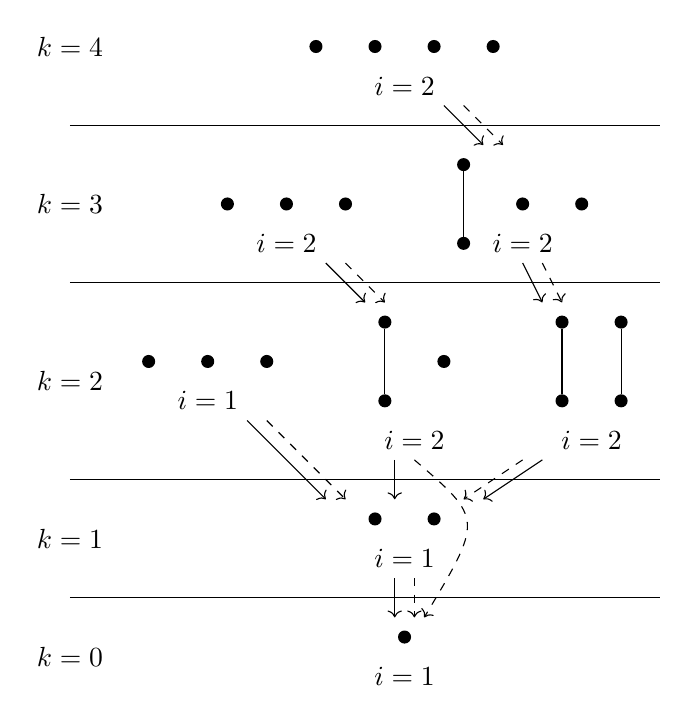
\begin{tikzpicture}

  % Level k = 4
  \node at (-1, 8) {$k=4$};

  \node[circle,fill=black,scale=0.5] (k4_1) at (2.125 + 0 * 0.75, 8) {};
  \node[circle,fill=black,scale=0.5] (k4_2) at (2.125 + 1 * 0.75, 8) {};
  \node[circle,fill=black,scale=0.5] (k4_3) at (2.125 + 2 * 0.75, 8) {};
  \node[circle,fill=black,scale=0.5] (k4_4) at (2.125 + 3 * 0.75, 8) {};
  \node at (2.125 + 0.75 * 1.5, 7.5) {$i=2$};

  \draw[->, dashed] (4, 7.25) -- (4.5, 6.75);
  \draw[->] (3.75, 7.25) -- (4.25, 6.75);

  \draw (-1, 7) -- (6.5, 7);

  % Level k = 3
  \node at (-1, 6) {$k=3$};

  \node[circle,fill=black,scale=0.5] (k3_1) at (1 + 0 * 0.75, 6) {};
  \node[circle,fill=black,scale=0.5] (k3_2) at (1 + 1 * 0.75, 6) {};
  \node[circle,fill=black,scale=0.5] (k3_3) at (1 + 2 * 0.75, 6) {};
  \node at (1 + 0.75, 5.5) {$i=2$};

  \draw[->, dashed] (2.5, 5.25) -- (3, 4.75);
  \draw[->] (2.25, 5.25) -- (2.75, 4.75);

  \node[circle,fill=black,scale=0.5] (k3_4) at (4 + 0 * 0.75, 6.5) {};
  \node[circle,fill=black,scale=0.5] (k3_5) at (4 + 0 * 0.75, 5.5) {};
  \node[circle,fill=black,scale=0.5] (k3_6) at (4 + 1 * 0.75, 6) {};
  \node[circle,fill=black,scale=0.5] (k3_7) at (4 + 2 * 0.75, 6) {};
  \draw (k3_4) -- (k3_5);
  \node at (4 + 0.75, 5.5) {$i=2$};

  \draw[->, dashed] (5, 5.25) -- (5.25, 4.75);
  \draw[->] (4.75, 5.25) -- (5, 4.75);

  \draw (-1, 5) -- (6.5, 5);

  % Level k = 2
  \node at (-1, 3.75) {$k=2$};

  \node[circle,fill=black,scale=0.5] (k2_1) at (0 + 0 * 0.75, 4) {};
  \node[circle,fill=black,scale=0.5] (k2_2) at (0 + 1 * 0.75, 4) {};
  \node[circle,fill=black,scale=0.5] (k2_3) at (0 + 2 * 0.75, 4) {};
  \node at (0 + 0.75, 3.5) {$i=1$};

  \draw[->, dashed] (1.5, 3.25) -- (2.5, 2.25);
  \draw[->] (1.25, 3.25) -- (2.25, 2.25);

  \node[circle,fill=black,scale=0.5] (k2_4) at (3 + 0 * 0.75, 3.5) {};
  \node[circle,fill=black,scale=0.5] (k2_5) at (3 + 0 * 0.75, 4.5) {};
  \node[circle,fill=black,scale=0.5] (k2_6) at (3 + 1 * 0.75, 4) {};
  \draw (k2_4) -- (k2_5);
  \node at (3 + 0.75 * 0.5, 3) {$i=2$};

  \draw[->, dashed] (3.375, 2.75) .. controls (4.25, 2) .. (3.5, 0.75);
  \draw[->] (3.125, 2.75) -- (3.125, 2.25);

  \node[circle,fill=black,scale=0.5] (k2_7) at (5.25 + 0 * 0.75, 3.5) {};
  \node[circle,fill=black,scale=0.5] (k2_8) at (5.25 + 0 * 0.75, 4.5) {};
  \node[circle,fill=black,scale=0.5] (k2_9) at (5.25 + 1 * 0.75, 3.5) {};
  \node[circle,fill=black,scale=0.5] (k2_10) at (5.25 + 1 * 0.75, 4.5) {};
  \draw (k2_7) -- (k2_8);
  \draw (k2_9) -- (k2_10);
  \node at (5.25 + 0.75 * 0.5, 3) {$i=2$};

  \draw[->, dashed] (4.75, 2.75) -- (4, 2.25);
  \draw[->] (5, 2.75) -- (4.25, 2.25);

  \draw (-1, 2.5) -- (6.5, 2.5);

  % Level k = 1
  \node at (-1, 1.75) {$k=1$};

  \node[circle,fill=black,scale=0.5] (k1_1) at (2.875 + 0 * 0.75, 2) {};
  \node[circle,fill=black,scale=0.5] (k1_2) at (2.875 + 1 * 0.75, 2) {};
  \node at (2.875 + 0.75 * 0.5, 1.5) {$i=1$};

  \draw[->, dashed] (3.375, 1.25) -- (3.375, 0.75);
  \draw[->] (3.125, 1.25) -- (3.125, 0.75);

  \draw (-1, 1) -- (6.5, 1);

  % Level k = 0
  \node at (-1, 0.25) {$k=0$};

  \node[circle,fill=black,scale=0.5] (k0_1) at (3.25, 0.5) {};
  \node at (3.25, 0) {$i=1$};
\end{tikzpicture}

  \caption{Search tree for $n = 4$ and $i = 2$.
    Level $k$ contains all posets that can be solved in $k$ comparisons and contribute to the solution for the given parameters $n$ and $i$.
    Solid arrows indicate predecessors, while dashed arrows represent the resulting problem when the reversed comparison is inserted.}
  \label{fig:backward-search-tree}
\end{figure}


\subsubsection{Predecessor calculation.} \label{sec:backward:predecessor_calculation}
We begin with a formal definition of a predecessor.

\begin{definition}[Predecessor] \label{definition:predecessor_calculation}
  The problem $(Q, j)$ is a \emph{predecessor} of $(P, i)$ if there is a comparison $(a, b)$ such that:
  \begin{enumerate}
    \item $(P, i) = \reduced(\pchild{Q}{a}{b}, j)$, and
    \item $V_j(\pchild{Q}{b}{a}) \leq V_i(P)$.
  \end{enumerate}
\end{definition}

Note that the first condition implies $V_i(P) = V_j(\pchild{Q}{a}{b})$.

Any problem $(Q, j)$ satisfying the first condition of the above definition is called a \emph{potential predecessor}.
In fact, the first step in enumerating the predecessors is to enumerate the potential predecessors.
The second step is to check the second condition.

\begin{lemma} \label{lemma:predecessor_calculation}
  Let $(P, i)$ and $(Q, j)$ be reduced problems, where $(Q, j)$ is a predecessor of $(P, i)$.
  Then, $V_j(Q) \leq V_i(P) + 1$.
\end{lemma}

\begin{proof} \label{proof:predecessor_calculation}
  Since $(Q, j)$ is a predecessor of $(P, i)$, $(a, b)$ exists with $\reduced{(\pchild{Q}{a}{b}, j)} = (P, i)$ and $V_j(\pchild{Q}{b}{a}) \leq V_i(P)$.
  Therefore, $V_j(Q) \leq \max\{V_j(\pchild{Q}{a}{b}), V_j(\pchild{Q}{b}{a})\} + 1 = V_i(P) + 1$.
\end{proof}

Storing only reduced problems presents a significant challenge to predecessor enumeration.
To illustrate this, consider a problem $(P, i)$ and its predecessor $(Q, j)$.
We know there exists a comparison $(a, b)$ such that $(P, i) = \reduced(\pchild{Q}{a}{b}, j)$.
However, it is possible that the edge $(a, b)$ is not present in $P$ because either $a$ or $b$ could have been removed during the reduction process.
The question arises: How can we undo a comparison that is not visible?
Furthermore, even if $a$ and $b$ are not removed during the reduction, there may be other elements that are removed.
The challenge is to determine how many elements are removed and what their relationships are.

To address these challenges, we will prove two lemmas.
The first lemma shows that after adding a comparison $(a, b)$, at most one of $\{a, b\}$ will be removed by the reduction.

\begin{lemma} \label{lemma:remove_only_last_element_edge}
  If $(P, i)$ is a reduced problem and $(Q, j) = \reduced{(\pchild{P}{a}{b}, i)}$, then, $\Omega_Q \cap \{a, b\} \neq \emptyset$.
\end{lemma}

\begin{proof}
  Since $(P, i)$ is reduced, we have $|\less{P}{c}| \leq i$ and $|\greater{P}{c}| \leq n - i + 1$, where $n = |\Omega_P|$, for every $c \in P$.
  In particular, this holds for both $a$ and $b$.
  Let $P' = \pchild{P}{a}{b}$ and assume $Q \cap \{a, b\} = \emptyset$.
  Observe that $\less{P'}{a} = \less{P}{a} \leq i$ and $\greater{P'}{b} = \greater{P}{b} \leq n - i + 1$.
  Thus, for $a$ and $b$ to be removed, we must have $\greater{P'}{a} \geq n - i + 2$ and $\less{P'}{b} \geq i + 1$.
  Note that there are no elements between $a$ and $b$, as they are incomparable in $P$ and there is a Hasse arc between them in $P'$.
  Hence, $\greater{P'}{a} \cap \less{P'}{b} = \{a, b\}$, leading to the contradiction $n = |\Omega_{P'}| \ge |\greater{P'}{a} \cup \less{P'}{b}| = |\greater{P'}{a}| + |\less{P'}{b}| - |\greater{P'}{a} \cap \less{P'}{b}| \ge n + 1$.
\end{proof}

The next lemma shows that the elements removed by the reduction, which are not $a$ or $b$, can be added one after the other in such a way that all the intermediate problems are reduced.
\Cref{fig:lemma_viz_example} exemplifies that this is not trivial -- a specific order is necessary for the intermediate problem to be reduced.

\begin{figure}[t]
{
  \centering
  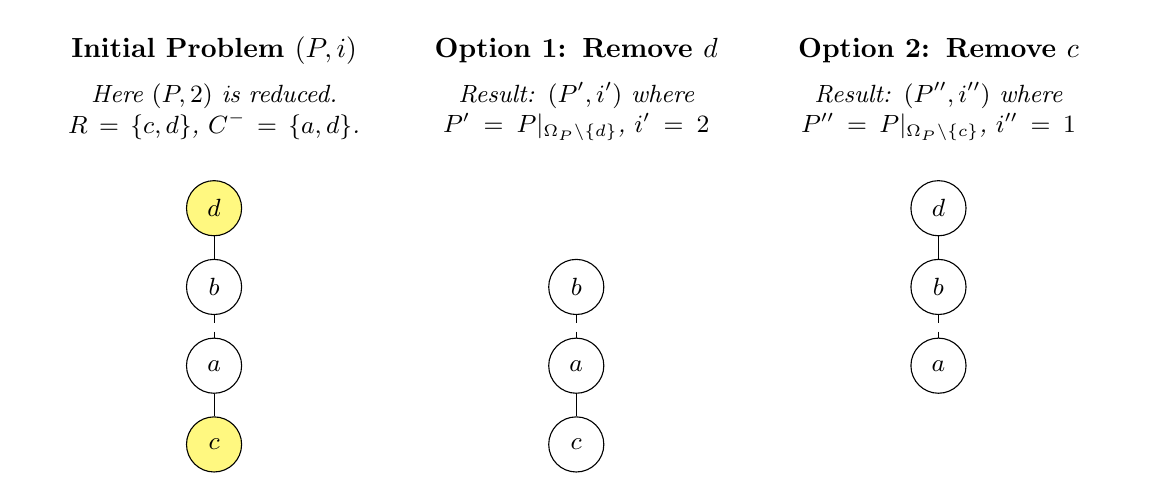
\begin{tikzpicture}[
    xscale=0.8, yscale=0.8,
    Pnode/.style={draw, circle, minimum size=7mm, inner sep=0pt, font=\small},
    Rnode/.style={Pnode, fill=yellow!50},
    labelnode/.style={font=\small\itshape, align=center, text width=4.5cm},
    descr/.style={font=\small, align=center, text width=4.5cm},
    mainlabel/.style={font=\bfseries, align=center, text width=4.5cm},
    arrowlabel/.style={midway, font=\scriptsize, text width=1.8cm, inner sep=0pt, align=center}
  ]

    \begin{scope}[xshift=0cm]
      \node[mainlabel] (P_title) at (0,0) {Initial Problem $(P, i)$};
      \node[labelnode, below=0.0cm of P_title] (P_i_val) {Here $(P, 2)$ is reduced. $R = \{c, d\}$, $C^-=\{ a, d \}$.};

      \node[Rnode] (d1) at (0,-2.5) {$d$};
      \node[Pnode] (b1) at (0,-3.75) {$b$};
      \node[Pnode] (a1) at (0,-5) {$a$};
      \node[Rnode] (c_el1) at (0,-6.25) {$c$};

      \draw (d1) -- (b1);
      \draw[dashed] (b1) -- (a1);
      \draw (a1) -- (c_el1);

    \end{scope}

    \begin{scope}[xshift=5.75cm]
      \node[mainlabel] (Pprime_title) at (0,0) {Option 1: Remove $d$};
      \node[labelnode, below=0.0cm of Pprime_title] (Pprime_i_val) {Result: $(P', i')$ where $P' = P|_{\Omega_P \setminus \{d\}}$, $i' = 2$};

      \node[Pnode] (b2) at (0,-3.75) {$b$};
      \node[Pnode] (a2) at (0,-5) {$a$};
      \node[Pnode] (c_el2) at (0,-6.25) {$c$};

      \draw[dashed] (b2) -- (a2);
      \draw (a2) -- (c_el2);

    \end{scope}

    \begin{scope}[xshift=11.5cm]
      \node[mainlabel] (Pdoubleprime_title) at (0,0) {Option 2: Remove $c$};
      \node[labelnode, below=0.0cm of Pdoubleprime_title] (Pdoubleprime_i_val) {Result: $(P'', i'')$ where $P'' = P|_{\Omega_P \setminus \{c\}}$, $i'' = 1$};

      \node[Pnode] (d3) at (0,-2.5) {$d$};
      \node[Pnode] (b3) at (0,-3.75) {$b$};
      \node[Pnode] (a3) at (0,-5) {$a$};

      \draw (d3) -- (b3);
      \draw[dashed] (b3) -- (a3);

    \end{scope}

  \end{tikzpicture}}

{\small
The problem $(Q, j)$ is obtained from $(P, i)$ by adding $a < b$ (the dashed edge) and reducing.
We have $(Q, j) = \reduced(\pchild{P}{a}{b}, i) = \reduced(\pchild{P'}{a}{b}, i') = \reduced(\pchild{P''}{a}{b}, i'')$ and $R = \Omega_P \setminus (\Omega_Q \cup \{a, b\}) = \{c, d\}$.
The problem $(P', i')$ is reduced, but $(P'', i'')$ is not.
}

  \caption{
    Example for \Cref{lemma:remove_elements_iteratively}.
  }
  \label{fig:lemma_viz_example}
\end{figure}

\begin{lemma} \label{lemma:remove_elements_iteratively}
  Let $(P, i)$ be a reduced problem, and let $(Q, j) = \reduced{(\pchild{P}{a}{b}, i)}$.
  If $(P, i)$ is a predecessor of $(Q, j)$ and $\Omega_P \setminus (\Omega_Q \cup \{a, b\})$ is not empty, then there exists an element $c \in \Omega_P \setminus (\Omega_Q \cup \{a, b\})$ such that $(P|_{\Omega_P \setminus \{c\}}, i')$, where $i' = i - 1$ if $|\greater{\pchild{P}{a}{b}}{c}| \ge n - i + 2$ and $i' = i$ otherwise, is a reduced predecessor of $(Q, j)$.
\end{lemma}

\begin{proof}
  Let $R = \Omega_P \setminus (\Omega_Q \cup \{a, b\})$ be the set of elements, other than $a$ or $b$, removed by the reduction.
  It is easy to see that for every $c \in R$, the problem $(P', i')$ where $P' = P|_{\Omega_P \setminus \{c\}}$ and $i' = i - 1$ if $|\greater{\pchild{P}{a}{b}}{c}| \ge n - i + 2$ and $i' = i$ otherwise is a predecessor of $(Q, j)$:
  \begin{itemize}
    \item It is obvious that $(Q, j) = \reduced{(\pchild{P'}{a}{b}, i')}$.
    \item The problem $(\pchild{P'}{b}{a}, i')$ cannot be harder than $(\pchild{P}{b}{a}, i)$, hence $V_{i'}(\pchild{P'}{b}{a}) \leq V_i(\pchild{P}{b}{a})$.
  \end{itemize}
  The challenge is to find an element $c$ such that $P'$ is reduced.
  We define the following sets:
  \begin{align*}
    C^+ & = \{e \in \Omega_P \mid |\greater{P}{e}| = n - i + 1\}            \\
    C^- & = \{e \in \Omega_P \mid |\less{P}{e}| = i \}                      \\
    R^+ & = \{c \in R \mid |\greater{\pchild{P}{a}{b}}{c}| \ge n - i + 2 \} \\
    R^- & = \{c \in R \mid |\less{\pchild{P}{a}{b}}{c}| \ge i + 1 \}
  \end{align*}
  Note that $R = R^- \cup R^+$.
  The elements in $C^-$ and $C^+$ are critical:
  If $P'$ is not reduced, it is because one of these elements can no longer be the $i'$-th smallest.
  To avoid this, we need an element $c \in R^+$ that is smaller (in $P$) than all elements in $C^-$.
  By symmetry, any element $c \in R^-$ larger than all elements in $C^+$ works as well.
  We first show that if we have an element in $R^- \cap C^-$ or $R^+ \cap C^+$, then this is the case as
  \begin{equation}
    \forall c \in C^+, e \in C^- \colon c \le_P e\,\text{.}
  \end{equation}
  Assume we have $c \in C^+$ and $e \in C^-$, but $c \not\le_P e$.
  Then the sets $\greater{P}{c}$ and $\less{P}{e}$ are disjoint, leading to the contradiction $|\greater{P}{c}| + |\less{P}{e}| = n + 1 > |\Omega_P|$.

  The second step is to show that if $R^- \cap C^- = \emptyset$ and $R^+ \cap C^+ = \emptyset$, we can pick any $c \in R$.
  We show:
  \begin{equation}
    \forall c \in R^-, e \in C^+ \colon e \le_P c \text{ or } e \in R^+\,\text{.}
  \end{equation}
  Assume we have $c \in R^-$ and $e \in C^+$.
  By another counting argument we observe that the sets $\less{\pchild{P}{a}{b}}{c}$ and $\greater{P}{e}$ cannot be disjoint:
  Assuming $\less{\pchild{P}{a}{b}}{c} \cap \greater{P}{e} = \emptyset$ leads to the contradiction $|\less{\pchild{P}{a}{b}}{c}| + |\greater{P}{e}| \ge n + 2$.
  Thus, $(e, c) \in \pchild{P}{a}{b}$.
  Hence, we have either $e \le_P c$ or $e \le_P a$.
  If $e \le_P a$ but $e \not\le_P c$, we have to show $a \neq e$ to conclude $e \in R^+$.
  Assume $a = e$.
  Then $\greater{P}{a} \setminus \{ a \}$ and $\less{\pchild{P}{a}{b}}{c}$ must be disjoint, as $e \not\le_P c$.
  We obtain the contradiction $|\greater{P}{a} \setminus \{ a \}| + |\less{\pchild{P}{a}{b}}{c}| \ge n + 1$.
  By symmetry, we also obtain:
  \begin{equation}
    \forall c \in R^+, e \in C^- \colon c \le_P e \text{ or } e \in R^-\,\text{,}
  \end{equation}
  which concludes the proof.
\end{proof}

The set of predecessors for a given problem $(P, i)$ can be split into the following three subsets, which we compute in that order.
\begin{enumerate}
  \item Predecessors on the same set of elements.
  \item Predecessors with exactly one additional element that is involved in the comparison.
  \item Predecessors with additional elements of which at least one is not part of the comparison.
\end{enumerate}
Of the predecessors to the problems in $A_k$, those that actually require $k+1$ comparisons (those not in $A_k$) make up the set $A_{k+1}$.
We describe the steps to compute the three sets below.

\subparagraph{Predecessors on the same set of elements.}
Our goal is to find all posets with $n$ elements that result in poset $P$ after inserting a comparison $a < b$.
Each edge in the Hasse diagram of $P$ potentially represents a comparison by which $(P, i)$ can be obtained from a predecessor.
A challenge arises from transitive relations, as the insertion of a single comparison can lead to the insertion of multiple transitive relations.
This is illustrated in \Cref{fig:backward_problematic}.
Removing a comparison from (1) can result in either (2) or (3).
Therefore, both (2) and (3) are potential predecessors, even though the same comparison is removed each time.

\begin{figure}[!b]
  \centering
  \begin{tikzpicture}
  \node[circle,draw=black] (A1) at (0, 0) {};
  \node[circle,draw=black] (A2) at (0, 1) {};
  \node[circle,draw=black] (A3) at (0, 2) {};

  \draw (A1) -- (A2) node {};
  \draw (A2) -- (A3) node {};
  \node (AL) at (0, -0.5) {$i = 1$};
  \node (A) at (0, -1) {(1)};


  \node[circle,draw=black] (B1) at (2.5 + 0, 0) {};
  \node[circle,draw=black] (B2) at (2.5 + 0, 2) {};
  \node[circle,draw=black] (B3) at (2.5 + 1, 1) {};

  \draw (B1) -- (B2) node {};
  \node (BL) at (2.5 + 0.5, -0.5) {$i = 1$};
  \node (B) at (2.5 + 0.5, -1) {(2)};


  \node[circle,draw=black] (C1) at (5 + 1, 2) {};
  \node[circle,draw=black] (C2) at (5 + 0, 0) {};
  \node[circle,draw=black] (C3) at (5 + 2, 0) {};

  \draw (C1) -- (C2) node {};
  \draw (C1) -- (C3) node {};
  \node (CL) at (5 + 1, -0.5) {$i = 1$};
  \node (C) at (5 + 1, -1) {(3)};
\end{tikzpicture}
  \caption{Case where further comparisons can be removed transitively by removing a comparison.}
  \label{fig:backward_problematic}
\end{figure}

After enumerating the potential predecessors, we check for each one whether it is a predecessor of $(P, i)$.
For a potential predecessor $(Q, j)$ where $(P, i) = \reduced{(\pchild{Q}{a}{b}, j)}$, we check whether $(\pchild{Q}{b}{a}, j)$ can be solved using at most $V_i(P)$ comparisons.
This is done by checking whether $\reduced{(\pchild{Q}{b}{a}, j)}$ is contained in one of the sets $A_k$ for $k \leq V_i(P)$, which have already been computed.


\subparagraph{Predecessors with exactly one additional element that is involved in the comparison.}
We construct the potential predecessor for this case as follows.
We add a new element to the poset $P$ and enumerate all possibilities for the relation between the new element and the existing elements.
We want the predecessor to be reduced, thus it is crucial to ensure that the new element cannot be immediately reduced and that no existing elements can be reduced either.
Since the new element is either smaller or larger than the $i$-th smallest element being searched for, either the $(i + 1)$-th smallest or the $i$-th smallest element is searched for in these predecessors.
Furthermore, for each $(Q, j)$ obtained this way, there must exist elements $a$ and $b$ such that $\reduced{(\pchild{Q}{a}{b}, j)} = (P, i)$.
This is required for $(Q, j)$ to be a potential predecessor, and since we additionally want the new element to be part of the comparison, we mandate that either $a$ or $b$ is the new element.
Checking whether the potential predecessors constructed this way are predecessors is done in the same way as in the preceding step.

For the correctness of our approach, note that if we have an arbitrary reduced predecessor, then by removing all elements that are not present in $P$, with the exception of $a$ and $b$, we obtain another reduced predecessor.
We get this by induction on the number of elements removed using \Cref{lemma:remove_elements_iteratively}.
If both $a, b \in \Omega_P$ then this predecessor is enumerated in the first step.
Otherwise, as proven in \Cref{lemma:remove_only_last_element_edge}, if one of $a$ or $b$ is in $\Omega_P$, the predecessor is enumerated in this second step.
In the next step, we will iteratively enumerate all predecessors by adding additional elements to the ones already found.
This way, we will discover the arbitrary predecessor we started with.

\subparagraph{Predecessors with additional elements of which at least one is not part of the comparison.}
Starting with the predecessors computed in the first two steps, new elements are iteratively inserted.
We alternate between generating new potential predecessors and checking which of those are actually predecessors.
We stop when no new predecessors are found or when we reach an upper limit on the number of elements.
New potential predecessors are generated by adding a new element to each predecessor and enumerating all possible relations with the existing elements.
When inserting a new element, it is important to note that it may no longer be the $i$-th smallest but rather the $(i + 1)$-th smallest element being searched, similar to the second step.
We only consider potential predecessors that are reduced and of cause by the addition of the comparison $a < b$ and subsequent reduction, the resulting problem $(P, i)$ should be obtained anew.

\subsubsection{Optimizations.}

\subparagraph{Limit search space.}
Each time an element is removed from a poset during reduction of a problem, a possible consequence is, that now we are looking for the $(i-1)$-th instead of the $i$-th element.
Therefore, if $(P, j)$ is a problem appearing in an algorithm selecting the $i$-th smallest of $n$ elements, then $i - j \le n - |\Omega_P|$.
An optimization we apply to the backward search is to ignore any problems that violate this inequality.
They cannot contribute to the solution.
E.g.\ no problem with $n=6$ and $i=2$ can lead to a problem with $n=7$, $i=4$.

\subparagraph{Iterative deepening.}
As the theoretical upper bounds are too high in practice, the program uses an iterative deepening approach.
It starts with an upper bound that corresponds to the theoretical lower bound, derived by \Cref{lemma:previous_next_poset} from the smaller values for $n$ and increments this bound until a solution is finally found.
As it is not possible to save which posets are ignored due to the guessed upper bound without considerable effort, the backward search is restarted several times.
Although results from previous rounds are not used, the search space can be considerably reduced, making the program more efficient.

\subparagraph{Remaining comparisons.}
This number of edges in the Hasse diagram of a poset is a lower bound to the number of comparisons that must be removed until the unordered poset is reached.
Since at most one comparison can be removed in each step, all posets containing too many Hasse arcs can be discarded, as they cannot lead to an unordered poset with the remaining comparisons.

\subparagraph{Parallelization.} \label{sec:backward:parallelisation}
The backward search can be ideally parallelized by performing the calculation of the predecessors in parallel.
The only two bottlenecks are read access to the cache and the efficient merging of all partial results.
As shown in \Cref{table:backward-parallel} for $n = 13$ and $i = 7$, it can be seen that the backward search scales well with the number of cores.
To set the different times in relation to the number of cores, the efficiency was determined, which represents a direct correlation between the two variables.
This can be calculated as follows
\[
  \text{efficiency} = \cfrac{\text{single-core time}}{\text{number of cores} \cdot \text{multi-core time}}\text.
\]
The higher the efficiency, the better the time scales with the number of cores.

\begin{table}[!t]
  \renewcommand{\arraystretch}{1.1}
  \caption{Efficiency of parallelism for $n = 13, i = 7$}
  \label{table:backward-parallel}
  \centering
  \small
  \begin{tabular}{l|rrrrrr}
    \textbf{cores}      & $1$    & $2$    & $3$    & $6$    & $12$   & $24$   \\ \hline
    \textbf{time} (m)   & 165    & 84     & 64     & 32     & 17     & 9      \\ \hline
    \textbf{efficiency} & $1.00$ & $0.99$ & $0.90$ & $0.87$ & $0.81$ & $0.75$
  \end{tabular}
\end{table}

\section{Results}

\begin{table}[!t]
  \renewcommand{\arraystretch}{1.1}
  \caption{Minimum number of comparisons needed to select the $i$-th smallest of $n$ elements.
    Values resulting from our work are printed in bold.}
  \label{table:num-comparisons}
  \centering
  \small
  \begin{tabular}{c|cccccccc}
    $n$ & \multicolumn{8}{c}{$i$}                                                                                                    \\
        & 1                       & 2  & 3           & 4           & 5           & 6           & 7                & 8                \\ \hline
    1   & 0                                                                                                                          \\
    2   & 1                                                                                                                          \\
    3   & 2                       & 3                                                                                                \\
    4   & 3                       & 4                                                                                                \\
    5   & 4                       & 6  & 6                                                                                           \\
    6   & 5                       & 7  & 8                                                                                           \\
    7   & 6                       & 8  & 10          & 10                                                                            \\
    8   & 7                       & 9  & 11          & 12                                                                            \\
    9   & 8                       & 11 & 12          & 14          & 14                                                              \\
    10  & 9                       & 12 & 14          & 15          & 16                                                              \\
    11  & 10                      & 13 & 15          & 17          & 18          & 18                                                \\
    12  & 11                      & 14 & 17          & 18          & 19          & 20                                                \\
    13  & 12                      & 15 & 18          & 20          & 21          & 22          & 23                                  \\
    14  & 13                      & 16 & 19          & 21          & 23          & 24          & \textbf{25}                         \\
    15  & 14                      & 17 & 20          & 23          & \textbf{24} & \textbf{26} & \textbf{26}      & \textbf{27}      \\
    16  & 15                      & 18 & \textbf{21} & \textbf{24} & \textbf{26} & \textbf{27} & \textbf{28} - 33 & \textbf{28} - 36 \\
  \end{tabular}
\end{table}

Running our computer search, we obtained the values $V_i(n)$ shown in \Cref{table:num-comparisons}.
Our findings confirm most of the values computed by Oksanen~\cite{Oksanen}.
Notably, $V_5(12) = 19$ contradicts a conjecture by Gasarch~\cite{Gasarch1996} that the optimum can be achieved using a ``pair-forming algorithm'', where the first comparison of any singleton is with another singleton (in this case, the best pair-forming algorithm requires 20 comparisons).
The values printed in bold were unknown previously.
For $V_7(14)$, $V_6(15)$, $V_7(15)$, and $V_8(15)$, only a range was known prior.
Oksanen incorrectly lists $V_5(15)$ as 25 on his website~\cite{Oksanen}, although his search algorithm does produce the correct value of 24.
The values for $n = 16$ have not been computed before; we provide all values for $i \leq 6$ and ranges for $V_7(16)$ and $V_8(16)$.
The upper bound for the ranges is $V_i(n) \le n - i + (i - 1) \lceil \log (n + 2 - i) \rceil$~\cite{hadian1969selecting}.

To validate the upper bounds of the values we calculated, we checked the algorithm certifying each number on each of the $n!$ permutations.
For the lower bound we computed each number twice using two different algorithms, the forward and the backward search.
This reduces the likelihood of an incorrect result due to a coding error.

\begin{table}[!t]
  \caption{Execution times and number of posets stored in the cache for different search methods.}
  \label{table:search_algorithms}
  \label{table:cache_entries}
  \begin{minipage}{\linewidth}
    \renewcommand{\arraystretch}{1.1}
    \centering
    \small
    \begin{tabular}{cc|ll|ll|l}
          &     & \multicolumn{2}{c|}{\textbf{Forward Search}} & \multicolumn{2}{c|}{\textbf{Backward Search}} & \textbf{Oksanen}                                                                                                                 \\
      $n$ & $i$ & {\footnotesize time}                         & {\footnotesize posets}                        & {\footnotesize time} & {\footnotesize posets} & {\footnotesize time}                                                             \\
      \hline
      12  & 6   & 1m 30s                                       & $1.9 \cdot 10^6$                              & 18.0s                & $996 \cdot 10^3$       & 1.9s
      \\
      \hline
      13  & 7   & 59m 20s                                      & $67.6 \cdot 10^6$                             & 7m 16s               & $14.5 \cdot 10^6$      & 16h 10m                                                                          \\
      \hline
      14  & 7   & 14h 40m                                      & $925.3 \cdot 10^6$                            & 2h 17m               & $263.3 \cdot 10^6$     & >5d\footnote{\label{fn:oksanen_abort}We aborted Oksanen's program after 5 days.} \\
      \hline
      15  & 8   & 14d 21h 26m                                  & $15.7 \cdot 10^9$                             & 1d 3h 7m             & $2.2 \cdot 10^9$       & >5d\footref{fn:oksanen_abort}                                                    \\
      \hline
      16  & 6   & 6d 11h 21m                                   & $3.6 \cdot 10^9$                              & 1d 1h 26m            & $2.6 \cdot 10^9$       & -                                                                                \\
    \end{tabular}
  \end{minipage}
\end{table}


\Cref{table:search_algorithms} compares the execution times of the different algorithms to find optimal selection algorithms.
All experiments were conducted on a machine with two Intel Xeon CPUs, each equipped with $12$ cores ($24$ threads), and a total of $768$ GB of RAM.
The forward search was started with $500$ GB of RAM and restarted for each combination of $n$ and $i$, ensuring no use of cached data from previous runs to provide comparability.
The `Oksanen' column presents execution times of Oksanen's program~\cite{Oksanen} on our hardware, started with a cache size of $25$ GB RAM.
It was originally designed to use $400$ MB RAM and $25$ GB is close to a natural limit due to the use of 32-bit indices.
Additionally, we measured the number of posets stored in the cache after the calculation, which can be found in \Cref{table:cache_entries}.

To evaluate the potential of compatible solutions as pruning criterion, we determined the maximum number of compatible solutions encountered for a given cost for $n \leq 14$ and used that as a boundary in a subsequent run.
For $n = 14, i = 7$, this resulted in a time of 1h~21m with $147 \cdot 10^6$ posets in the cache -- improvements by factors of $11$ and $6.3$, respectively.


\section{Conclusion and Open Questions}


As stated in the motivation before: the road is better than the inn.
Along the way we improved the forward search using a pruning criterion based on compatible solutions and evaluated a new algorithmic approach -- the backward search coming to a final conclusion that both are valid.
Between the structural constraints of our algorithms and the available hardware, $n=16$ is likely the limit of feasible calculation for the current state.
We believe that higher $n$ are realistic with new algorithmic ideas and conclude this work by talking about promising directions for further research.
The latest version of our software is available at \projectServer~(\url{\projectURL}).

\subparagraph{Bidirectional Search.}
The classical meet-in-the-middle approach for a bidirectional search will not work for the selection problem.
Our experiments with the forward and backward search showed that, using the number of comparisons as metric, at any possible meeting point, at least one of the two searches has already covered over $99\%$ of its search space.

An alternative approach to the bidirectional search would be to first run the backward search, but restricted to problems with specific properties such as having a large number of compatible solutions, e.g.\ problems $(P, i)$ in $A_k$ with $\mathcal{C}(P, i) \ge \alpha \cdot 2^k$ for some $\alpha \in [0, 1]$.
These are presumably hard to solve, so the subsequent forward search only has to explore problems with a small number of compatible solutions, which should be easier to solve.

There might be better metrics than the compatible solutions, as there is a significant gap between the lower bound and the cost of a problem.
We observed that the number of comparisons required to solve a selection problem is typically about twice the lower bound obtained from the number of compatible solutions, minus a constant.
This observation is reasonable, as the lower bound for the median is $n + \smallO(n)$, which is far from the best known asymptotic lower bound $2n + \smallO(n)$.

\subparagraph{Improved Weight Function.}
A better lower bound might be achieved by assigning a weight to each solution rather than merely counting compatible solutions.
Mimicking the techniques used to obtain the $2n + \smallO(n)$ bound in~\cite{bent1985finding} could be a fruitful approach.

\subparagraph{Yao's conjecture.}
Yao conjectured that finding the $i$-th smallest of $n$ elements is at least as hard as finding an $n$-element subset $S$ of $m$ elements, where $m > n$, and an element $s \in S$ such that $s$ is the $i$-th smallest element in $S$~\cite{yao1974lower}.
If true, it would imply a $2.5n + \smallO(n)$ algorithm for computing the median~\cite{schonhage1975finding}.
By adapting our search algorithm, one could search for counter examples to the conjecture.


\bibliography{lipics-v2021-sample-article}
  

\end{document}
